\chapter{Unity DOTS: NetCode}
\label{cap:netcode}
Assieme allo sviluppo dell'architettura data-oriented introdotta con DOTS, si è reso necessario implementare dei meccanismi che permettessero di utilizzare il modello di ECS anche nella comunicazione in rete.
Il package NetCode permette di realizzare un design di rete a server dedicato con predizione lato client, in cui lo scambio di messaggi avviene tramite entità, componenti e sistemi. Il funzionamento di NetCode si basa su API di più basso livello fornite dal package Transport, il quale sostituisce la vecchia libreria di Unity per il networking.
In questo capitolo forniremo un'infarinatura sullo sviluppo di videogiochi multiplayer assieme ad un background sulle possibili problematiche introdotte con il networking. Infine, mostreremo le soluzioni proposte e le scelte attuate da Unity per la realizzazione dei package DOTS relativi al multiplayer.

\section{Background sullo sviluppo di giochi multiplayer}
Quando parliamo di sviluppo di giochi multiplayer è necessario avere ben chiaro in mente come funziona la comunicazione in Internet e scegliere la soluzione migliore per il tipo di gioco che si vuole realizzare. A tal proposito è importante conoscere le principali topologie di rete, i protocolli utilizzati ed i problemi che possono occorrere.

\subsubsection{Topologie di rete}
I videogiochi multiplayer possono essere strutturati in diversi modi, ognuno dei quali con i propri vantaggi e svantaggi, ed ognuno adatto a tipi di giochi differenti.

\paragraph{Locale}
È la tipologia più semplice. Il gioco esegue su una singola macchina, di conseguenza l'unico codice da implementare è quello del client. La differenza rispetto ad un videogioco singleplayer è che il gioco in locale riceve e deve processare diversi input, in quanto ci sono più giocatori. Tra i vantaggi di questa topologia di rete spiccano la latenza prossima a zero, la sicurezza e la complessità minima del modello. Tuttavia, è una soluzione poco scalabile in quanto di norma non consente la partecipazione di più di 4 giocatori, i quali devono trovarsi nella stessa stanza. Dunque, solitamente viene utilizza per giochi semplici, quali platform e puzzle games in schermo condiviso o split screen~\cite{youtube:realtime-multiplayer}.

\paragraph{LAN}
Anche questo modello è offline ma, al contrario del precedente, permette di connettere diversi dispositivi. Ai vantaggi dei giochi in locale aggiunge la scalabilità: infatti, tramite questa soluzione è possibile raggiungere anche centinaia di giocatori. In ogni caso, persiste il problema che i partecipanti devono essere vicini e raggiungibili. Ultimamente viene utilizzata soprattutto per i giochi che utilizzano la realtà virtuale, in quanto è necessaria una latenza minima~\cite{youtube:realtime-multiplayer}.

\paragraph{Peer-to-peer}
È una topologia di rete che sfrutta la connessione ad Internet, in cui tutti i giocatori che partecipano alla sessione di gioco sono collegati fra loro. Poiché ogni peer ha \emph{O(n - 1)} connessioni, dove \emph{n} è il numero di peer, questa soluzione è poco scalabile, in quanto maggiore è il numero di peer collegati, maggiore sarà la banda di rete richiesta. Inoltre, con questa soluzione vi è \emph{input sharing}, ovvero ogni peer deve ricevere e processare gli input di tutti gli altri. Di conseguenza, è necessario mantenerli sincronizzati per evitare che la latenza di uno provochi il disallineamento delle simulazioni di gioco. Ciò rende la logica alla base di questo modello sorprendentemente complessa da implementare. Solitamente questa soluzione viene utilizzata in giochi in cui le partite vengono disputate fra un numero ristretto di partecipanti~\cite{book:multiplayergameprogramming}.

\paragraph{Client$/$Server}
il design di questa rete prevede una separazione del codice di gioco fra client e server. Ogni client comunica solo con il server, mentre il server deve comunicare con tutti i client collegati. Quindi, il server deve mantenere \emph{O(n)} connessioni, dove \emph{n} è il numero di client, mentre ogni client mantiene una sola connessione, verso il server. Fra i vantaggi di questa soluzione vi è il fatto che i client non devono processare gli input di tutti gli altri client, ma ricevono solo gli aggiornamenti del server. Inoltre, la banda richiesta non aumenta con il numero di client, se non di valori irrilevanti dovuti alle dimensioni dello stato di gioco ricevuto (più client ci sono, più oggetti da replicare dovranno essere trasmessi)~\cite{book:multiplayergameprogramming}.

\paragraph{Sottocategorie}
Oltre a queste macro categorie esistono anche delle sottocategorie, in particolare per il modello Client/Server.
Un'architettura di tipo \emph{Listen server} è un modello a Client/Server in cui un client diventa server e ospita la partita per tutti gli altri client. I problemi principali consistono nel fatto che l'host è privilegiato in quanto non ha latenza. Di conseguenza, è necessario implementare un sistema di migrazione dell'host in caso questo si disconnetta, creando situazioni spiacevoli in cui tutti devono aspettare.

\begin{figure}[!ht]
    \begin{subfigure}{.49\textwidth}
      \centering
      % include first image
      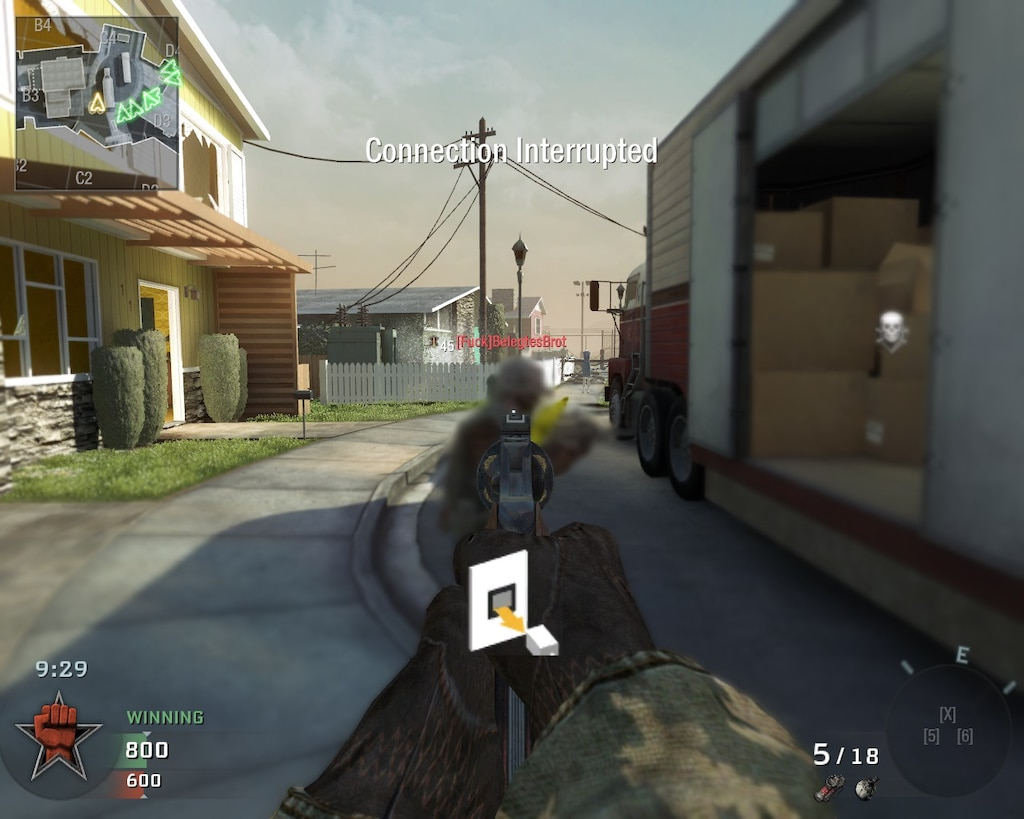
\includegraphics[width=.95\linewidth]{gfx/imgs/chapter3/CoDBOConnectionInterrupted.png}
      \caption{Connessione Interrotta.}
      \label{fig:connection-interrupted}
    \end{subfigure}
    \begin{subfigure}{.49\textwidth}
      \centering
      % include second image
      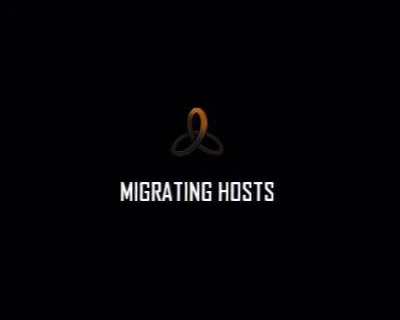
\includegraphics[width=.95\linewidth]{gfx/imgs/chapter3/CoDBO2MigratingHosts.png}
      \caption{Migrazione Host.}
      \label{fig:host-migration}
    \end{subfigure}
    \caption{Esempi di problemi di connessione nei giochi multiplayer con riferimento a Call of Duty.}
    \label{fig:multiplayer-problems}
\end{figure}

Nel modello a \emph{Server dedicato} vengono utilizzati server ospitati, solitamente forniti da servizi di hosting, per cui il controllo è totalmente nelle mani dello sviluppatore, invece che dei giocatori. Questo permette di fare delle scelte specifiche in base al target del gioco, ad esempio possiamo scegliere server più o meno potenti e distribuirli maggiormente in giro per il mondo man mano che il gioco cresce in popolarità. Tipicamente questa soluzione prevede che il server sia headless, ovvero non sfrutta alcuni moduli quali il sistema di rendering grafico, in quanto non ha bisogno di renderizzare nulla ma solo mantenere in esecuzione la simulazione principale.

Esiste inoltre il modello a \emph{Server autoritativo}, nel quale vengono eseguiti due tipi di simulazione, ma l'unica da considerare sempre corretta è quella del server. Di conseguenza, se per qualche motivo il client dovrebbe trovarsi in uno stato incerto, aggiornerà il proprio stato in base a ciò che riceve dal server. Ciò limita molto la possibilità di utilizzo di hack o cheat per ottenere vantaggi rispetto agli altri giocatori~\cite{book:multiplayergameprogramming, youtube:realtime-multiplayer}.

Gli ultimi due modelli solitamente vengono utilizzati insieme e rappresentano una soluzione estremamente scalabile, ideale per giochi le cui partite vengono disputate da un numero di partecipanti molto elevato, ad esempio i battle royale, che possono arrivare anche a più di 100 giocatori connessi contemporaneamente. Fra gli svantaggi principali vi sono: i costi, in quanto per progetti di grandi dimensioni solitamente è necessario affidarsi a servizi di hosting o data center; la latenza dovuta al fatto che, essendo i client connessi fra di loro indirettamente tramite il server, i messaggi devono prima passare da quest'ultimo, per essere ricevuti dagli altri. Per questo motivo solitamente si cerca di implementare un sistema di matchmaking che privilegi le connessioni fra client ``limitrofi''.
Il modello a server dedicato autoritativo è di particolare interesse ai fini della tesi, in quanto rappresentano l'architettura scelta da Unity per lo sviluppo della nuova libreria di networking introdotta con DOTS.

\begin{figure}[!ht]
    \begin{subfigure}{.49\textwidth}
      \centering
      % include first image
      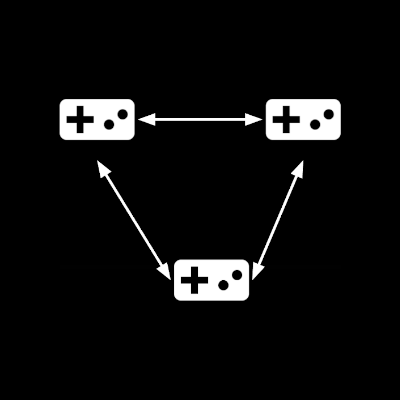
\includegraphics[width=.95\linewidth]{gfx/imgs/chapter3/PeerToPeerSchema.png}
      \caption{Peer-to-peer.}
      \label{fig:peer-to-peer}
    \end{subfigure}
    \begin{subfigure}{.49\textwidth}
      \centering
      % include second image
      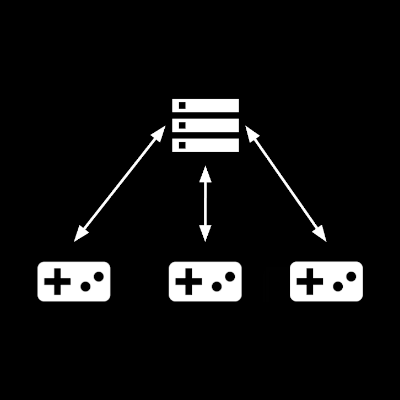
\includegraphics[width=.95\linewidth]{gfx/imgs/chapter3/DedicatedServerSchema.png}
      \caption{Server dedicato.}
      \label{fig:dedicated-server}
    \end{subfigure}
    \caption{Schemi delle connessioni dei due modelli più utilizzati.}
    \label{fig:authoritative-server}
\end{figure}

\subsubsection{Transport layer e protocolli UDP e TCP}
Nello sviluppo di un videogioco multiplayer, il livello più basso dello stack di rete con cui è possibile sporcarsi le mani è il transport layer (tutto il resto viene svolto dall'architettura sottostante e dall'hardware). A questo livello si trovano le socket, che permettono di stabilire un canale di comunicazione tra due end-point e utilizzano due protocolli principali:

\paragraph{TCP}
È orientato alla connessione e garantisce affidabilità, ovvero che i pacchetti arrivino sempre, in ordine e senza essere duplicati. Per questo motivo i pacchetti TCP hanno un header pesante (le dimensioni variano da 20 a 60 byte) che contiene diverse informazioni, molte delle quali sono inutili ai fini del gioco che si vuole implementare. Inoltre, per come è realizzato TCP, nel caso un pacchetto venga perso, viene richiesta una ritrasmissione e questo genera latenza extra assolutamente non tollerabile in un gioco in tempo reale. Come se ciò non bastasse, con TCP la perdita di pacchetti c'è sempre, poiché dispone di un meccanismo di controllo di congestione, il cui algoritmo prevede che la velocità di trasmissione aumenti sempre finché non viene perso un pacchetto, per poi diminuire e ricominciare ad aumentare gradualmente~\cite{standard:rfc5681}.

\paragraph{UDP}
È leggero e molto più veloce, in quanto non dà alcun tipo di garanzia e, di conseguenza, ha un header di dimensioni ridotte (8 byte). Infatti, con questo protocollo i pacchetti non vengono tracciati e, nel caso un pacchetto venga perso, nessuno se ne accorge e la comunicazione continua. Nel caso fossero necessarie particolari specifiche di affidabilità, bisognerebbe implementarle manualmente.

\paragraph{Cosa scegliere}
Poiché in un videogioco l'aspetto più importante è garantire un'esperienza di gioco ottimale per tutti, la scelta del protocollo assume particolare rilevanza. Solitamente utilizziamo TCP solo nei giochi a turni, perché la latenza non permette di avere una risposta soddisfacente da parte del server. Dunque, la scelta più gettonata è UDP, a cui di norma aggiungiamo l'implementazione di qualche tecnica per evitare che i pacchetti vengano riordinati, arrivino duplicati, oppure vengano persi.

\subsubsection{Problematiche di rete nei videogiochi multiplayer}
Indipendentemente dal tipo di gioco, per quanto la tecnologia si sia evoluta negli ultimi decenni, possono verificarsi comunque dei problemi dovuti ai limiti fisici dell'hardware (schede di rete obsolete, router eterogenei, cavi datati) e alla velocità con cui possono essere trasmessi i dati (connessioni limitate, banda di rete condivisa).
Per questo motivo è importante progettare l'applicazione tenendo conto delle diverse problematiche che possono avere un impatto negativo sull'esperienza di gioco.
\paragraph{Latenza, Jitter e Perdita di pacchetti}
Quando un gioco viene testato in rete locale alcuni dei fattori che influenzano negativamente il gioco non sono presenti. Quando però il gioco viene rilasciato, possono verificarsi i seguenti:
\begin{itemize}
    \item Latenza. Si riferisce al tempo che impiega un pacchetto ad essere trasferito dal nodo sorgente a quello di destinazione. Questo ritardo impone un limite inferiore alla velocità con cui le informazioni e lo stato di gioco possono essere scambiate fra due end-point, condizionando di conseguenza la possibilità dei giocatori di reagire a cambiamenti situazionali.
    \item Jitter. consiste nella variazione di latenza fra un pacchetto ed il seguente. Questo può essere un problema ad esempio per i giocatori (o anche per il game engine stesso) che non riescono a compensare la latenza a medio o lungo termine della rete.
    \item Perdita di pacchetti. si verifica quando un pacchetto non raggiunge mai la destinazione. Se degli aggiornamenti dello stato del gioco vengono persi, il game engine deve sistemare il danno come meglio può per fare in modo che la simulazione non risulti compromessa e sia comunque fluida e giocabile.
\end{itemize}

Le cause di queste problematiche possono essere differenti. Sebbene molte siano dovute a limiti hardware non risolvibili, altre possono essere aggirate o attenuate tramite l'utilizzo di particolari tecniche o meccanismi implementativi durante lo sviluppo dell'applicazione.
Inoltre, a seconda del tipo di gioco che stiamo sviluppando, le problematiche definite precedentemente possono incidere in modi differenti, più o meno tollerabili. Ad esempio, una latenza considerevole, di addirittura 500ms, è accettabile in alcuni RTS\footnote{Nei giochi \emph{Real-Time Strategy} il giocatore solitamente controlla delle unità assegnandovi delle azioni da svolgere.}, mentre generi come gli FPS, i MOBA\footnote{Nei \emph{First-Person Shooter} e \emph{Multiplayer Online Battle Arena}, il giocatore controlla un singolo personaggio, dunque è necessaria una risposta molto rapida ai comandi.} ed i picchiaduro necessitano di valori attorno ai 30ms (in generale non oltre i 50ms), per non rovinare l'esperienza di gioco~\cite{book:networkingandonlinegames, book:multiplayergameprogramming}.

\paragraph{Tecniche per migliorare la latenza}
La latenza è un problema che esiste sempre e non è possibile eliminarlo a priori. Tuttavia, possiamo utilizzare delle tecniche per aggirarla e migliorare, almeno in parte, l'esperienza di gioco. Ad esempio, poiché il flusso di gioco solitamente non è costante (gli aggiornamenti inviati dal server non arrivano con la stessa frequenza), questo potrebbe causare una percezione fastidiosa da parte del giocatore, che vedrebbe il gioco eseguire a scatti. A tal proposito esiste una tecnica chiamata \emph{interpolazione lato client}, che permette di smussare il flusso di gioco. Ciò allevia la sensazione di latenza che questa condizione genera, rendendo il gioco più fluido. Infatti, tramite questo metodo, quando il client riceve uno stato dal server non lo presenta subito, ma calcola l'interpolazione tra l'ultimo stato ricevuto ed il precedente, utilizzando un filtro di percezione locale.

Tuttavia, l'interpolazione migliora l'esperienza di gioco, ma non avvicina ciò che il giocatore vede a ciò che effettivamente sta succedendo lato server. Anche se il periodo di interpolazione fosse breve, lo stato di gioco sarebbe comunque più vecchio di 1/2 RTT\footnote{Round Trip Time (RTT): somma del tempo che impiega un pacchetto a transitare in rete dal nodo mittente al ricevente ed il tempo che impiega il pacchetto di risposta (ad esempio un ACK che conferma la ricezione) a tornare sul nodo iniziale. Si misura in millisecondi.} rispetto a quello del server.

Per riuscire a mostrare uno stato di gioco che sia più corretto, è necessario utilizzare la \emph{predizione lato client}, che viene attuata tramite l'estrapolazione. Per farlo è necessario che il client esegua la stessa simulazione del server e, quando riceve un aggiornamento da quest'ultimo, sa che è datata di 1/2 RTT. Dunque, per rendere lo stato più corretto, il client esegue la simulazione per un ulteriore 1/2 RTT. Così facendo, quando il client presenta la simulazione al giocatore, è un'approssimazione molto più veritiera di ciò che sta effettivamente succedendo lato server. Per mantenere l'approssimazione, il client continua ad eseguire la simulazione ogni frame e mostrare il risultato al giocatore. Poi, quando riceve un nuovo stato dal server, internamente lo simula per 1/2 RTT che, idealmente, a questo punto corrisponde allo stato esatto che il client ha già calcolato in base al precedente~\cite{book:multiplayergameprogramming}.

\subsubsection{Soluzione proposta da Unity}
Con l'introduzione di DOTS, la vecchia libreria per il networking UNet è diventata obsoleta e serviva qualcosa di più adeguato all'architettura basata sul modello orientato ai dati di ECS. A tal proposito Unity ha inserito nello stack due package, con l'obbiettivo di realizzare una comunicazione performante e scalabile (sul modello di DOTS), che fosse compatibile fra piattaforme eterogenee e che fosse, inoltre, modulare e trasparente:
\begin{itemize}
    \item \textbf{Transport}. Questo package è implementato sfruttando il protocollo UDP, in quanto estremamente semplice e veloce, aggiungendovi però alcune funzionalità. In particolare, sono state inserite utilità per: pacchettizzare i dati da inviare ad ogni frame di gioco, tramite un buffer; gestire le connessioni, permettendo di avere qualche garanzia in più ad esempio sul fatto che il server esista effettivamente, oppure che si ottenga una notifica in caso il server vada offline o non sia più raggiungibile; integrare il sistema di networking con il job system di unity, permettendo di eseguire le simulazioni di rete su thread multipli oppure, anche nel caso in cui si stia utilizzando un server a thread singolo, ottenere tutti i benefici della compilazione con burst~\cite{youtube:unity-transport}.
    \item \textbf{NetCode}. Questo package è stato pensato per sviluppare principalmente giochi in tempo reale, i quali impongono requisiti di latenza contenuta. A tal proposito è stato realizzato sul modello a server dedicato con server autoritativo, utilizzando le API fornite dal Transport package. Per attenuare il problema della latenza è stata introdotta la predizione lato client. In questo modo l'esperienza di gioco risulta fluida e piacevole~\cite{youtube:unity-netcode}.
\end{itemize}

%%%%%%%%%%%%%%%%%%%%%%%%%%%%%%%%%%%%%%%%%%%%%%%%%%%%%%%%%%%%%%%%%%%%%%%%%%%%%
% roba più pratica con costrutti e come funzionano spiegati nel dettaglio
\section{Transport package}
Il package \emph{Transport} (com.unity.transport) è stato realizzato per sostituire le API di basso livello della vecchia libreria UNet per il networking, ormai diventata obsoleta. Contiene costrutti e metodi utili alla serializzazione degli stream di dati da inviare in rete, permettendo di stabilire connessioni e spedire messaggi ad host remoti.

\subsubsection{Scambio di messaggi}
La comunicazione in questo package si basa su un modello ad eventi, i quali danno informazioni sullo stato della connessione (ad esempio indicano se ci sono messaggi da leggere). I dati vengono trasmessi in rete a blocchi e, quando si vuole costruire un sistema di comunicazione, è necessario tenere conto dell'allineamento in memoria e dell'ordine dei byte (Endianness), il quale può variare fra dispositivi eterogenei~\cite{doc:microsoft-memory-alignment, youtube:unity-transport}. Per questo motivo, il Transport package fornisce dei costrutti che permettono di bufferizzare i dati senza dover tenere in considerazione tutte queste convenzioni, in quanto l'implementazione sottostante fa già tutto per noi:
\begin{itemize}
    \item \verb|DataStreamWriter|. Permette di allocare un buffer di memoria e supporta scritture di tipo deferred. È possibile utilizzarlo per serializzare i dati da inviare ed essendo una struttura non è gestito da un garbage collector.
    \item \verb|DataStreamReader|. È la controparte del precedente e permette di deserializzare i dati ricevuti. È ciò che si ottiene quando si riceve un evento dalla rete e permette di leggere i dati ricevuti, accumulati in un buffer. Al contrario del precedente è una struttura \emph{immutabile}. Di conseguenza, tutto lo stato contenuto dev'essere memorizzato in un context esterno, altrimenti non sarebbe possibile aggiornare la posizione di lettura e bisognerebbe specificare gli offset dei byte manualmente (operazione estremamente prona ad errori).
\end{itemize}

\subsubsection{Gestione delle connessioni}
Per realizzare lo scambio di messaggi tra due endpoint si utilizza la struttura \verb|NetworkDriver|, che implementa le connessioni virtuali a livello del transport layer sia per i client che per il server(host).
Una connessione virtuale è rappresentata da una struttura \verb|NetworkConnection|, che mantiene tutte le informazioni necessarie al driver per comunicare con l'altro endpoint ed è ottenibile connettendosi ad un server oppure accettando una connessione.

\paragraph{NetworkDriver}
\verb|NetworkDriver| è il costrutto principale del package e sfrutta l'interfaccia di rete \verb|INetworkInterface| che rappresenta la socket di basso livello, per inviare e ricevere dati. Contiene metodi per creare il driver, eseguire il binding (con UNet questo veniva fatto in automatico), connettersi a un server dal client, accettare le connessioni dei client dal server, inviare e ricevere dati da una connessione, eseguire l'operazione di pop (ovvero leggere e rimuovere) dalla coda degli eventi di rete~\cite{doc:unity-transport-api}.

Infatti, poiché lo scambio di messaggi tra i driver di due endpoint viene notificato tramite eventi, la struttura \verb|NetworkDriver| dispone di 4 tipi di eventi differenti, contenuti nell'enumerativo \verb|NetworkEvent.Type|:
\begin{itemize}
    \item \verb|Empty| (default). Indica che non ci sono altri messaggi da leggere nella coda degli eventi, per il frame corrente.
    \item \verb|Data|. Indica che sono stati ricevuti dei dati da un endpoint connesso ed è possibile leggerli mediante \verb|DataStreamReader|.
    \item \verb|Connect|. Indica che è stata stabilita una nuova connessione (disponibile solo se il driver non si trova in stato listening).
    \item \verb|Disconnect|. Indica che è stato ricevuto un pacchetto di disconnessione, si è verificato un timeout della socket, oppure è stato raggiunto il limite massimo di tentativi di connessione a \verb|NetworkConnection|.
\end{itemize}

Questi eventi sono i medesimi sia per client che per server, l'unica differenza è come vengono consumati~\cite{doc:unity-transport-manual}.

Inoltre, il driver dispone di un metodo \verb|BeginSend()| che restituisce una struttura \verb|DataStreamWriter|, utilizzabile per inviare dati all'altro endpoint della connessione specificata.

Solitamente la sequenza di esecuzione del codice è:
\begin{enumerate}
    \item Il client invia un evento \verb|Connect| al server.
    \item Il server risponde con un evento \verb|ConnectionAccept|.
    \item Sia server che client possono iniziare subito a trasmettere dati.
    \item Il server invia un evento \verb|Disconnect| e la comunicazione termina.
\end{enumerate}

Poiché il transport package è realizzato utilizzando UDP, è possibile che un pacchetto venga perso. Nel caso venisse perso il messaggio \emph{Connect}, è presente un timeout dopo il quale, se non viene ricevuta risposta dal server, ne viene inviato un altro. Così facendo ci si assicura che la connessione venga effettivamente stabilita. Nel caso a essere perso fosse, invece, il messaggio \emph{ConnectionAccept}, avviene una connessione implicita, con cui il client capisce che la connessione è stata accettata, al primo pacchetto contenente dei dati ricevuto dal server.

Il motivo per cui non è possibile inviare dati prima della conferma della connessione, è dovuto al fatto che il package Transport supporta connessioni multiple dei client al medesimo server. Di conseguenza, è necessario un meccanismo per identificare le connessioni dei vari client e che le mantenga ``up-to-date'': ogni client assieme al messaggio di richiesta della connessione invia un token identificiativo, al quale il server risponde col proprio token. Senza la conoscenza dei reciproci token, la comunicazione non può avvenire~\cite{youtube:unity-transport}.

\subsubsection{Integrazione con Unity Job System}
Il package Transport è stato realizzato per essere compatibile col modello di ECS e con il job system: i costrutti principali sono infatti strutture blittable, che permettono di ottenere tutti i benefici offerti dalla tecnologia DOTS, fra cui la possibilità di utilizzare il burst compiler.
A tal proposito, è possibile scaricare il lavoro del network driver, che normalmente verrebbe svolto tutto sul main thread, in job secondari, permettendo di dedicare più spazio (in un frame) alla logica di gioco. Inoltre, è anche possibile gestire le varie connessioni in parallelo, sfruttando un job di tipo \verb|IJobParallelFor| assieme alla versione concorrente del driver \verb|NetworkDriver.Concurrent|.

Poiché \verb|NetworkDriver| viene aggiornato da un job (motivo per cui il metodo che lo esegue si chiama \verb|.ScheduleUpdate()|), è necessario aspettare che termini prima di utilizzare il driver per qualsiasi altra cosa, difatti solitamente viene effettuata una chiamata al metodo \verb|.Complete()| all'inizio del ciclo di update~\cite{doc:unity-transport-manual, youtube:unity-transport}.

%L'integrazione col job system permette di eseguire tutte le simulazioni in rete su thread multipli. Inoltre, anche se si sta utilizzando un server a thread-singolo, o per un qualsiasi motivo (magari risparmiare a livello economico, utilizzando meno risorse CPU) è necessario utilizzare un singolo core, utilizzare il Job System permette di compilare il codice con burst, ottenendo un ingente miglioramento di prestazioni.

%%%%%%%%%%%%%%%%%%%%%%%%%%%%%%%%%%%%%%%%%%%%%%%%%%%%%%%%%%%%%%%%%%%%%%%%%%%%%
\section{NetCode package}
Il package \emph{NetCode} (com.unity.netcode) fornisce un modello di rete a server dedicato con predizione lato client, utilizzabile per realizzare la parte multigiocatore di un videogioco. Si basa sulle API del package Transport per le funzionalità a livello di socket, il quale è stato realizzato per essere compatibile ed ottimizzato per ECS e job system.

Al contrario di Transport, NetCode è ancora in preview, ovvero gli sviluppatori Unity stanno lavorando per migliorarlo e aggiungere ulteriori funzionalità. Pertanto, non è ancora pronto per l'utilizzo in produzione, ma è già possibile usarlo nei propri progetti~\cite{doc:unity-netcode-manual}.

\subsection{Concetti fondamentali in NetCode}

NetCode separa la logica dei client da quella del server, utilizzando world differenti per ciascuno di essi. Infatti, mentre usando semplicemente il package Entities, Unity creava un world di default in cui inizializzava ed aggiornava i vari sistemi e gruppi, con NetCode questo world viene creato comunque ma non viene utilizzato (a meno che non venga specificato diversamente). Al suo posto si utilizzano ClientWorldN dove N è il numero del client corrispondente partendo da 0, e ServerWorld, rispettivamente per la logica dei client e la logica del server.
All'interno di questi si trovano i sistemi, organizzati in gruppi specifici per l'inizializzazione, la simulazione e la presentazione. Il gruppo relativo alla presentazione è presente solo nei world client, in quanto si occupa del rendering (un frame visibile a schermo corrisponde ad una chiamata alla \verb|OnUpdate()| di questo gruppo) e di tutte quelle operazioni che servono solo ai client.

\SaveVerb{PresentationSystemGroupTerm}|PresentationSystemGroup|

\begin{figure}[!ht]
    \begin{subfigure}{.49\textwidth}
      \centering
      % include first image
      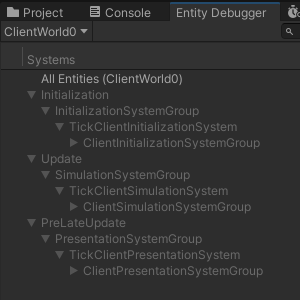
\includegraphics[width=.95\linewidth]{gfx/imgs/chapter3/SystemGroupClientNetCode.png}
      \caption{Gruppi principali nei ClientWorld.}
      \label{fig:client-world-groups}
    \end{subfigure}
    \begin{subfigure}{.49\textwidth}
      \centering
      % include second image
      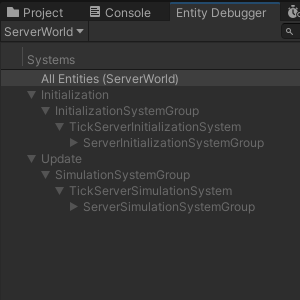
\includegraphics[width=.95\linewidth]{gfx/imgs/chapter3/SystemGroupServerNetCode.png}
      \caption{Gruppi principali nel ServerWorld.}
      \label{fig:server-world-groups}
    \end{subfigure}
    \caption{EntityDebugger: gerarchia dei gruppi principali a runtime (in ServerWorld non è presente il relativo \UseVerb{PresentationSystemGroupTerm}).}
    \label{fig:netcode-system-groups}
\end{figure}

%\paragraph{Bootstrap}
%La sequenza di bootstrap di default crea i world di client e server automaticamente all'avvio dell'applicazione, popolandoli con i sistemi definiti in base agli attributi impostati. Poiché, per vari motivi, può essere necessario ritardare la creazione dei mondi, NetCode permette di estendere la classe \verb|ClientServerBootstrap| per sovrascrivere la sequenza di bootstrap di default, fornendo metodi per la creazione del DefaultWorld e dei mondi di client e server manualmente.

\paragraph{RPC}
Le Remote Procedure Call (RPC) permettono di effettuare una chiamata ad una procedura che verrà eseguita su un dispositivo remoto. NetCode utilizza una forma limitata delle RPC per gestire degli eventi: un job che esegue sull'endpoint del mittente invia una richiesta di RPC ed un job che esegue sul lato destinatario la riceve chiamandone la funzione.

\paragraph{Ghost}
Un ghost è un networked object, ovvero un'entità simulata dal server ma trasmessa e aggiornata in tutti i client tramite delle snapshot (gli stati del gioco). Il client li presenta ma non ci può interagire direttamente perché appartengono al server.
Per creare un ghost è necessario aggiungere ad un entità i componenti \verb|GhostAuthoringComponent| e, in caso si voglia abilitare la predizione dell'entità solo per il client a cui appartiene (e interpolarlo per gli altri), \verb|GhostOwnerAuthoringComponent|~\cite{doc:unity-netcode-api}.

\paragraph{Condivisione dei dati fra client e server}
Per condividere delle entità fra client e server si utilizza lo stesso metodo utilizzato senza networking: inserendo i GameObject all'interno di una subscene, questi vengono convertiti in entità, che saranno presenti in tutti i world client e nel world server.\\
Per condividere i ghost, è necessario creare una oggetto che ne mantenga la lista: tramite il componente \verb|GhostCollectionAuthoringComponent|, il sistema che gestisce i ghost può identificarli fra client e server~\cite{doc:unity-netcode-manual}.

\paragraph{Multiplayer PlayMode Tools}
Quando si eseguono i test per un videogioco in locale, non sono presenti tutte le problematiche dovute alla connessione, che potrebbero invece verificarsi una volta pubblicato. A tal proposito NetCode mette a disposizione uno strumento che permette impostare come l'applicazione si deve comportare quando si entra in Play Mode nell'editor. Tramite questa finestra è possibile eseguire in uno stesso processo su Unity il codice del server, del client o entrambi, aggiungere dei \emph{client leggeri} e simulare i principali problemi di rete: latenza, jitter e perdita di pacchetti.

\begin{figure}[!ht]
    \centering
    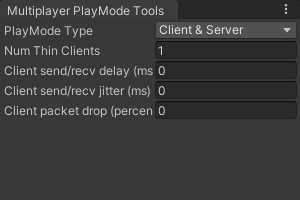
\includegraphics[width=0.50\columnwidth]{gfx/imgs/chapter3/MultiplayerPlayModeTools.png}
    \caption{Finestra \emph{Multiplayer PlayMode Tools}.}
    \label{fig:multiplayer-playmode-tools}
\end{figure}

\subsection{Stabilire una connessione}
\label{subsec:netcode-stabilire-connessione}
La connessione alla rete utilizza il Transport package ed immagazzina le connessioni come entità. Ogni entità connessione presenta un componente \verb|NetworkStreamConnection| che contiene una struttura \verb|NetworkConnection|.
Affinché la comunicazione venga avviata ed il server possa iniziare ad inviare snapshot ai client (ovvero gli stati del gioco), dopo aver ottenuto un riferimento a \verb|NetworkStreamReceiveSystem|, è necessario che:
\begin{enumerate}
    \item Il server entri in stato listening per ricevere richieste di connessione su una porta, chiamando il metodo \verb|Listen()| sul sistema.
    \item Un client si connetta al server, chiamando il metodo \verb|Connect()| sul sistema (a questo punto client e server sono connessi tramite una socket UDP).
    \item Il server marchi tutte le connessioni come ``in gioco'', tramite il componente \verb|NetworkStreamInGame| (ora client e server possono comunicare tramite comandi e snapshot)~\cite{doc:unity-netcode-manual}.
\end{enumerate}

Per richiedere una disconnessione è necessario aggiungere un componente \verb|NetworkStreamRequestDisconnect| all'entità che rappresenta la connessione. Dopodiché a questa viene aggiunto il componente \verb|NetworkStreamDisconnect| per un frame ed infine avviene effettivamente la disconnessione (l'entità viene eliminata)~\cite{youtube:unity-netcode}.

\begin{lstlisting}[caption={Prototipo: stabilimento della connessione.}, label={lst:example-connection},language={[Sharp]C}]
#region Stabilimento connessione

// itera su tutti i mondi presenti
foreach (var world in World.All) 
{
    var network = world.GetExistingSystem<NetworkStreamReceiveSystem>();
    // Codice eseguito nel caso ci troviamo in ClientWorld#
    if (world.GetExistingSystem<ClientSimulationSystemGroup>() != null) 
    {
        world.EntityManager.CreateEntity(typeof(EnableGame));
        NetworkEndPoint ep = NetworkEndPoint.LoopbackIpv4;
        ep.Port = 7979;
        network.Connect(ep); // Connect
    }
    // Codice eseguito nel caso ci troviamo in ServerWorld
    else if (world.GetExistingSystem<ServerSimulationSystemGroup>() != null) 
    {
        world.EntityManager.CreateEntity(typeof(EnableGame));
        NetworkEndPoint ep = NetworkEndPoint.AnyIpv4;
        ep.Port = 7979;
        network.Listen(ep); // Listen
    }
}

#endregion
\end{lstlisting}

\subsection{Comunicazione in NetCode}
Dopo aver stabilito la connessione, è possibile far comunicare i client ed il server. In NetCode esistono principalmente tre modi per comunicare, tramite RPC, comandi oppure snapshot.

\subsubsection{Comunicazione tramite RPC}
\label{subsubsec:comunicazione-rpc}
In NetCode è possibile utilizzare le RPC basandosi sul modello di ECS. Per creare una RPC in NetCode è necessario creare un comando (eventualmente contenente dei campi, rigorosamente di tipo blittable), implementando l'interfaccia \verb|IRpcCommand|. Questa interfaccia estende semplicemente \verb|IComponentData|, senza aggiungervi nulla, ma serve per indicare a NetCode che si riferisce ad un comando RPC.

\begin{lstlisting}[caption={Esempio di comando RPC non contenente campi.}, label={lst:example-rpc-struct},language={[Sharp]C}]
public struct OurRpcCommand : IRpcCommand
{
}
\end{lstlisting}

Implementando questo comando, NetCode genera automaticamente il codice utile per la serializzazione, deserializzazione e registrazione della RPC (in caso fosse necessario è possibile implementarlo manualmente).

Poiché NetCode si basa su ECS, per utilizzare le RPC è necessario creare un'entità che invii il comando ed una che lo riceva. Ciò viene realizzato creando un'entità mittente e aggiungendovi il comando creato ed un componente \verb|SendRpcCommandRequestComponent|, il quale contiene una struttura \verb|NetworkConnection| relativa al destinatario. Nel caso del client non è necessario indicare a chi è diretta, in quanto l'unico endpoint con cui può comunicare è il server a cui è connesso. Al contrario, se il server volesse inviare una richiesta di RPC, dovrebbe specificare a quale connessione questa è diretta e, in caso venga impostata a \verb|Entity.Null|, il messaggio verrebbe inviato in broadcast a tutti i client connessi. Solitamente quanto descritto viene inserito nel codice della \verb|OnUpdate()| di un sistema.

\begin{lstlisting}[caption={Esempio di invio di un comando Rpc dal client.}, label={lst:example-rpc-client-system},language={[Sharp]C}]
#region Invio Rpc

var commandBuffer = new EntityCommandBuffer(Allocator.Temp);
var req = commandBuffer.CreateEntity();

// aggiunge il componente del comando RPC creato in precedenza
commandBuffer.AddComponent(req, new OurRpcCommand());

// indica a NetCode che vogliamo inviare la RPC al server
commandBuffer.AddComponent(req, new SendRpcCommandRequestComponent());
commandBuffer.Playback(EntityManager);

#endregion
\end{lstlisting}

Ciò che non vediamo è che nei world di client e server è presente un sistema \verb|RpcSystem| che rileva l'invio e la ricezione di richieste RPC: appena viene aggiunto il componente \verb|SendRpcCommandRequestComponent| ad un'entità, tale sistema invia la richiesta ed elimina l'entità nel mondo in cui è stata creata; sul lato del destinatario, invece, \verb|RpcSystem| crea un'entità con lo stesso comando \verb|IRpcCommand| ed un componente \verb|ReceiveRpcCommandRequestComponent|~\cite{doc:unity-netcode-manual}. A tal proposito, per rilevare la ricezione di una RPC in un sistema, possiamo iterare su tutte le entità che possiedono quel componente ed eliminarle una volta processati i dati, come vediamo in Codice~\ref{lst:example-rpc-server-system}.

\begin{lstlisting}[caption={Esempio di ricezione di un comando Rpc sul server.}, label={lst:example-rpc-server-system},language={[Sharp]C}]
#region Ricezione Rpc

var commandBuffer = new EntityCommandBuffer(Allocator.Temp);

// itera su tutte le entita' che hanno il comando Rpc creato ed il componente che
// indica la ricezione, il quale permette anche di capire quale client l'ha inviato.
Entities.ForEach((Entity entity, ref OurRpcCommand cmd,
    ref ReceiveRpcCommandRequestComponent req) => {
    
    // una volta ricevuta l'entita' dobbiamo distruggerla, altrimenti
    // l'espressione della lambda continua a fare match con lo stesso comando Rpc. 
    PostUpdateCommands.DestroyEntity(entity);
    
    // [...]
}).Run();
commandBuffer.Playback(EntityManager);

#endregion
\end{lstlisting}

\subsubsection{Stream di comandi}
I client inviano continuamente uno stream di comandi al server (che li riceve in un buffer specifico), che includono tutti gli input e gli ACK dell'ultima snapshot ricevuta. NetCode utilizza il sistema \verb|NullCommandSendSystem| per inviare ACK anche nel caso non vengano ricevuti nuovi comandi, così da mantenere attivo il flusso della comunicazione.

Per creare un nuovo tipo di comando è possibile implementare l'interfaccia \verb|ICommandData|, che eredita da \verb|IBufferElementData|, al cui interno è necessario fornire una proprietà per accedere al \verb|Tick|~\cite{doc:unity-netcode-api}.

\begin{lstlisting}[caption={Prototipo(client): comando per l'input del giocatore.}, label={lst:example-command-data},language={[Sharp]C}]
public struct PlayerInput : ICommandData
{
    public uint Tick { get; set; }
    public int horizontal;
    public int vertical;
}
\end{lstlisting}

Come per le RPC il codice per la serializzazione e deserializzazione viene generato automaticamente se non specificato manualmente.

Una volta creato il comando, è possibile creare un sistema che campioni gli input del giocatore, e li invii al server, appunto, sotto forma di comandi. Per fare ciò è necessario che gli input vengano accumulati in un buffer, prima di poter essere inviati al server, pertanto bisogna aggiungere un buffer, del nuovo tipo di comando creato, all'entità del giocatore (che può essere, ad esempio, il suo personaggio). Dopodiché, è necessario aggiungere il componente \verb|CommandTargetComponent| all'entità che rappresenta la connessione. Così è possibile fare in modo che il \verb|CommandTargetComponent| referenzi l'entità del giocatore, a cui è stato aggiunto il buffer per i comandi.

Quando si aggiungono comandi al buffer, è necessario aggiornare anche il valore di \verb|Tick|, con il valore di \verb|ServerTick|, ottenuto da \verb|ClientSimulationSystemGroup|. In questo modo il server potrà applicare l'input nel momento giusto alla simulazione e inviare
al client una snapshot corretta~\cite{doc:unity-netcode-manual}.

\begin{lstlisting}[caption={Prototipo(client): parte del sistema che campiona gli input del giocatore e li invia al server sotto forma di comandi.}, label={lst:example-command-input},language={[Sharp]C}]
#region Rilevazione input e Invio del comando al server

var localInput = GetSingleton<CommandTargetComponent>().targetEntity;

// [...]

var input = default(PlayerInput);
input.Tick = m_ClientSimulationSystemGroup.ServerTick;

// input del giocatore e aggiornamento del valore del comando
if (Input.GetKey("a"))
    input.horizontal -= 1;
if (Input.GetKey("d"))
    input.horizontal += 1;
if (Input.GetKey("s"))
    input.vertical -= 1;
if (Input.GetKey("w"))
    input.vertical += 1;

// aggiunta del comando al buffer
var inputBuffer = EntityManager.GetBuffer<PlayerInput>(localInput);
inputBuffer.AddCommandData(input);

#endregion
\end{lstlisting}

Per accedere agli input ricevuti dal client, è possibile creare un sistema lato server, che legga tali valori da un'entità contenente il buffer di comandi. La lettura dev'essere effettuata assolutamente tramite il metodo \verb|GetDataAtTick()| del buffer, che permette di ottenere il tick esatto in cui è stato inserito l'input dal client, altrimenti le simulazioni non corrisponderebbero e il gioco potrebbe comportarsi in modi imprevisti.

\begin{lstlisting}[caption={Prototipo(server): parte della lambda expression che aggiorna la velocità del personaggio del giocatore, all'interno del sistema che riceve i comandi.}, label={lst:example-command-output},language={[Sharp]C}]
#region Applicazione del comando al personaggio

PlayerInput input;
inputBuffer.GetDataAtTick(tick, out input);
var speed = pms.speed;

// aggiorna la velocita' del personaggio del giocatore
if (input.horizontal > 0)
    pv.Linear.x += speed * deltaTime;
if (input.horizontal < 0)
    pv.Linear.x -= speed * deltaTime;
if (input.vertical > 0)
    pv.Linear.z += speed * deltaTime;
if (input.vertical < 0)
    pv.Linear.z -= speed * deltaTime;
    
#endregion
\end{lstlisting}

Nel caso per la comunicazione fosse necessario inviare uno stream costante di dati da client a server, si consiglia di utilizzare \verb|ICommandData|, piuttosto che \verb|IRpcCommand|~\cite{doc:unity-netcode-api}. % API ICommandData - utilissimo

\subsubsection{Ghost snapshot}
Il sistema di ghost snapshot di NetCode invia aggiornamenti sullo stato di gioco sincronizzando le entità che esistono sul server, marcate come ghost, con tutti i client. Il server processa per chunk, mentre i client (coloro che ricevono le snapshot), processano per entità. Questo perché non è possibile processare per chunk su entrambi i lati ed il server necessità di un processamento più efficiente, in quanto mantiene più connessioni del client.

Il componente \verb|GhostAuthoringComponent| permette di modificare le impostazioni dei vari ghost, indicando se supporta l'interpolazione, la predizione o entrambe, e se dev'essere sempre interpolato, se vi dev'essere applicata la predizione di tutti o solo del client a cui appartiene. Quest'ultima opzione indica che in tutti i client a cui non appartiene il ghost esso verrà interpolato e, per essere applicata, necessita anche dell'aggiunta del componente \verb|GhostOwnerComponentAuthoring|, il cui campo \verb|NetworkId| dev'essere impostato dal codice per impostarne il proprietario.

\subsection{Predizione lato client}
Per implementare la predizione in un gioco multiplayer, il client deve eseguire la stessa simulazione del server. Così facendo, il client può applicare gli input direttamente al personaggio locale, riducendo notevolmente la latenza, e ricevere snapshot dal server per controllare che la simulazione sia corretta.

NetCode applica la predizione a tutte le entità che a tempo di esecuzione hanno il componente \verb|PredictedGhostComponent|. Questo componente viene aggiunto, dal sistema di conversione dei ghost \verb|GhostAuthoringConversion|, a tutti i ghost con la predizione abilitata sul client e a tutti i ghost, senza distinzione, sul server. Questo perché non serve predire un ghost interpolato se i dati vengono utilizzati solo dal client.
\verb|PredictedGhostComponent| contiene, lato client, informazioni sulla predizione, fra cui ad esempio quali snapshot sono state applicate al ghost.

Per applicare la predizione in un sistema è necessario aggiungere l'attributo \verb|[UpdateInGroup(typeof(GhostPredictionSystemGroup))]|. Questo gruppo esegue sempre ad un timestep fisso, per ottenere gli stessi risultati su client e server.

Poiché il ciclo di predizione esegue dall'ultimo tick applicato ad ogni entità e alcune potrebbero avere già nuovi dati, sul client è necessario controllare se queste devono essere simulate oppure no, utilizzando il metodo \verb|GhostPredictionSystemGroup.ShouldPredict()| prima di aggiornare un'entità: se restituisse un valore falso, il codice dell'aggiornamento non dovrebbe essere eseguito per tale entità.

Il ciclo di predizione del server esegue esattamente una sola volta, e non aggiorna la struttura \verb|TimeData| in quanto è già corretta. Ciononostante, imposta comunque \verb|GhostPredictionSystemGroup.PredictingTick| per assicurare che lo stesso esatto codice possa essere eseguito sia lato client che lato server.

\subsection{Sincronizzazione del tempo}
Poiché NetCode utilizza un modello a server autoritativo, il server esegue ad un timestep fisso basato su quanto tempo è passato dall'ultimo aggiornamento, mentre il client, ad eccezione del codice di predizione che esegue anch'esso sempre ad un timestep fisso, aggiorna ad un timestep dinamico. Affinché il modello funzioni, il client deve far corrispondere ogni volta il proprio tempo a quello del server.

A tal proposito il sistema \verb|NetworkTimeSystem| calcola quale tempo del server dev'essere presentato sul client, facendo una stima iniziale in base al RTT e all'ultima snapshot ricevuta dal client. Quando il client riceve una stima iniziale, apporta piccoli cambiamenti al tempo corrente, basandosi sul tempo trascorso da quanto arrivano i comandi sul server e quando vengono effettivamente utilizzati: ricevendo questo valore dal server, il client può aggiustare il proprio tempo in modo tale da ricevere aggiornamenti appena prima che gli servano.

In altre parole, quando il client invia dei comandi al server, questi arriveranno ad un certo punto in futuro. Quando il server li riceve, li applica alla simulazione, ma il client deve poter stimare a quale tick questo avverrà sul server, così da poter applicare anche lui l'input nello stesso momento della simulazione. A tal proposito, il client fa una stima del \emph{prediction tick}, ovvero il tick in cui il server applicherà i comandi nella sua simulazione (quella corretta), riuscendo ad ottenere un'approssimazione notevole.

Per gli oggetti interpolati il funzionamento è diverso: il client dovrebbe presentarli in uno stato per cui ne ha ricevuto i dati. Questo tempo viene chiamato \emph{interpolazione} e Unity lo calcola inserendo un offset al tempo di predizione. L'offset, chiamato \emph{interpolation delay}, viene aggiustato tramite piccoli incrementi e decrementi, per fare in modo che il tempo di interpolazione avanzi in modo fluido. Unity calcola l'interpolation delay in base al RTT ed al jitter in modo tale che questo dato sia generalmente sempre disponibile e, poiché il tempo aggiunto è basato sul tick rate della rete, è anche robusto ad eventuali perdite di pacchetti.
